\documentclass[a4paper,11pt,leqno,notitlepage,onecolumn]{article}
%\documentclass[a4paper,11pt,leqno,notitlepage,twocolumn]{article}

\usepackage[latin1]{inputenc}
\usepackage{fontenc}
\usepackage{graphicx}
\usepackage[dvips]{hyperref}
\usepackage{subfigure}
\usepackage{setspace}
\doublespacing

\begin{document}
\title{Efficient Static Binary Instrumentation for X86/X86\_64 on Linux}
\author{Michael Laurenzano, Mustafa Tikir, Laura Carrington, Allan Snavely\\
San Diego Supercomputer Center\\
\it{\{michaell, mtikir, laurac, allans\}@sdsc.edu}}
\date{}
\maketitle

\begin{abstract}
\begin{it}

Binary instrumentation enables insertion of additional code into an
executable in order to observe or modify the behavior of application runs. 
There are two main approaches to binary instrumentation: static and dynamic
binary instrumentation. In this paper, we present PMaC's instrumentation toolkit (PIX), 
an efficient static  instrumentation toolkit for Linux on x86/x86\_64 platforms. PIX
is similar to the other toolkits in terms of how additional code is inserted. However, it uses whole function level
code relocation in order to remedy the difficulty created by the variable-length instruction set. Code relocation of this kind allows the
instrumentation tool to reorganize the application code in such a way that it
can use the fast  far-reaching constructs to transfer control
from the application to the instrumentation code rather than relying on multiple
jumps or interrupts for the transfer. Furthermore, the PIX API provides a means to
tool developers to insert lightweight hand-coded assembly
rather than relying solely on the insertion of entire instrumentation functions.
PIX also enables implementation of efficient instrumentation tools, 
with overheads for basic block counting that are an
average of 1.6x less than the overhead imposed by Pin, 4.7x less than the overhead imposed by
DynamoRIO, 7.8x less than the overhead imposed by Valgrind, and 75.6x less than the overhead imposed by Dyninst.

\end{it}

\end{abstract}

\label{Section:Introduction}
\section{Introduction}
\label{sec:Introduction}

Binary instrumentation toolkits can be used to insert additional code into an
executable in order to observe or modify the behavior of application runs.
Instrumentation toolkits such as Pin\cite{luk2005pin},
Dyninst\cite{buck2000api}, Valgrind\cite{nethercote2007valgrind} and
DynamoRIO\cite{bruening2004efficient} have been widely used to gather
information about application runs. It has been shown that data gathered from
instrumentation tools can be effectively used in guiding hardware and system
design\cite{uhlig1997trace}, program debugging and
correctness\cite{nethercote2007shadow}, program
optimization\cite{romer1997instrumentation}, security
verification\cite{miller-playing}, and performance
modeling/prediction\cite{snavely2001modeling}.

There are two main approaches to binary instrumentation: \textit{static} and
\textit{dynamic} binary instrumentation. Static binary instrumentation inserts
additional information into an executable and generates a persistent modified
executable whereas the dynamic instrumentation inserts additional information
during execution without making any permanent modifications to the executable.
The static instrumentation approach can be advantageous because it usually
results in more efficient executables when compared to the dynamic approach.
This is a result of the fact that static instrumentation introduces only the
instrumentation code itself, which is also included in the text section of the
executable. In dynamic binary instrumentation, additional overhead is introduced
because the instrumentation tool must perform additional tasks such as parsing,
disassembly, code generation, and making other decisions at runtime.

This is simply not an issue with static binary instrumentation tools because all
decisions and actions are taken prior to runtime. The only cost born at runtime
is the direct cost of performing additional instrumentation. Unlike static
instrumentation, dynamic instrumentation uses the program heap for the
instrumentation code and hence, use the data section as text space. However,
static binary instrumentation has disadvantages. It is not possible to
instrument shared libraries unless the shared libraries are instrumented
separately and the executable is modified to use those instrumented libraries.
Static instrumentation also provides less flexibility to tool developers since
any instrumentation code that is inserted persists throughout the application
run while dynamic instrumentation provides the means to delete instrumentation
code when it is not needed \cite{tikir2002efficient}. However, there are cases
where the importance of efficiency is enough to outweigh other shortcomings
\cite{carrington2006performance} so that static binary instrumentation is the
desirable paradigm.   

In this paper we introduce \textbf{P}MaC's \textbf{E}fficient static
\textbf{B}inary \textbf{I}nstrumentation toolkit for \textbf{L}inux on
x86/x86\_64, \textit{PEBIL}. The goal of PEBIL is to provide a toolkit that
enables the construction of instrumentation tools that produce an efficient
instrumented executable. More specifically, PEBIL is designed to generate
efficient instrumented executables for instrumentation tools that require a
large number of instrumentation points because these are the situations where
efficiency is expected to be most impacted. Similar to previous instrumentation
toolkits \cite{buck2000api}, PEBIL instruments the executable by placing a jump
instruction at each instrumentation point in the application which transfers
control to the instrumentation code. This instrumentation code saves program
state, performs tasks requested by the instrumentation tool, restores program
state, and then returns control to the application. A typical binary
instrumentation tool on a platform with fixed-length instructions
\cite{tikir2006pmac} accomplishes initial control transfer by replacing a single
instruction at the instrumentation point with a jump that transfers control to
the instrumentation code. 

When instructions are variable-length, however, this strategy is not always
possible since there may not be enough space to correctly insert such a jump
instruction. To address this, PEBIL relocates and tranforms the code for each
function to ensure that enough space (in the form of \begin{it}nops\end{it}) is
available to hold a full-length branch instruction at each instrumentation
point. This method of function relocation enables transformation of the code so
that it can use longer-range yet efficient jump instructions to transfer control
from the application to the instrumentation code. Similar to Dyninst
\cite{buck2000api}, PEBIL uses the concept of an instrumentation
\textit{snippet}, which is a lightweight hand-written body of assembly code that
can be used to perform instrumentation tasks, rather than relying only on
heavyweight instrumentation functions.

The PEBIL toolkit, along with other accompanying tools and documentation, is
open source and available to the public for download at
\url{http://blankforblindreview.com/}. The distribution includes
several instrumentation tools including a function execution counter, a basic
block execution counter, and a memory address stream collection tool. Each of
these tools is built on top of an API that provides both enough low-level detail
to allow the tool developer to get involved in the details of the
instrumentation and enough high-level capability to allow the tool builder to
ignore these details if he wishes. The three instrumentation tools provided with
the distribution are implemented in less than 600 lines of C++ code. The
remainder of the paper is organized as follows. Section \ref{sec:Overview}
describes the design and implementation of PEBIL. Section \ref{sec:Efficiency}
discusses several aspects of the toolkit that are related to efficiency,
including the function relocation mechanism and the instrumentation snippet.
Section \ref{sec:Results} presents some experiments that expose the performance
penalties imposed by instrumenting applications with PEBIL, as well as a
comparison of PEBIL to other state of the art binary instrumentation toolkits
for x86 including Dyninst, Pin, Valgrind and DynamoRIO. Section \ref{sec:Future}
discusses the future of PEBIL, Section \ref{sec:Related} discusses other popular
instrumentation tools related to PEBIL and Section \ref{sec:Conclusions}
concludes.


\label{Section:Overview}
\section{Overview}

Static binary instrumentation generates a modified executable 
 that can be run at a later time. When the instrumented executable is
run, the extra instrumentation code is run
in addition to the original code of the program. In order to insert additional code
and data, additional space must be allocated within the executable in a way that it
will, at load-time, be treated by the system in a manner appropriate to its
purpose. 

Most compilers produce an ELF executable whose
structure is similar to that shown in Figure \ref{Figure:OrigExecutable}. By
convention, most executables use only two loadable segments and some of the Linux
implementations, such as FreeBSD, only allow two loadable segments. Thus, it is
preferable for us to incorporate instrumentation text and data into the
existing text and data segments of the application. The default in most
compilers is to place the text segment prior and adjacent to the data segment.
We therefore prepend the instrumentation text to the existing text
segment\footnote{The amount of space allocated prior to the text section is
controlled by the linker variable \_\_executable\_start. We have seen cases
where the system does not provide enough space prior to the text segment by
default, in which case we provide a set of tools that produces a modified linker
script that provides up to 128MB of space.} and append the instrumentation data to the
data segment (as shown in Figure \ref{Figure:InstExecutable}). This
scheme has the added benefit of causing no immediate disturbance to the
addresses of the existing text and data segments of the program.

\begin{figure}[ht]
\centering
\caption[Optional caption for list of figures]{\subref{Figure:OrigExecutable} and \subref{Figure:InstExecutable} show the prepending
of instrumentation text to the existing text, and the prepending of instrumentation data to the existing data respectively.}
\subfigure[The structure of an unmodified typical ELF file.]{
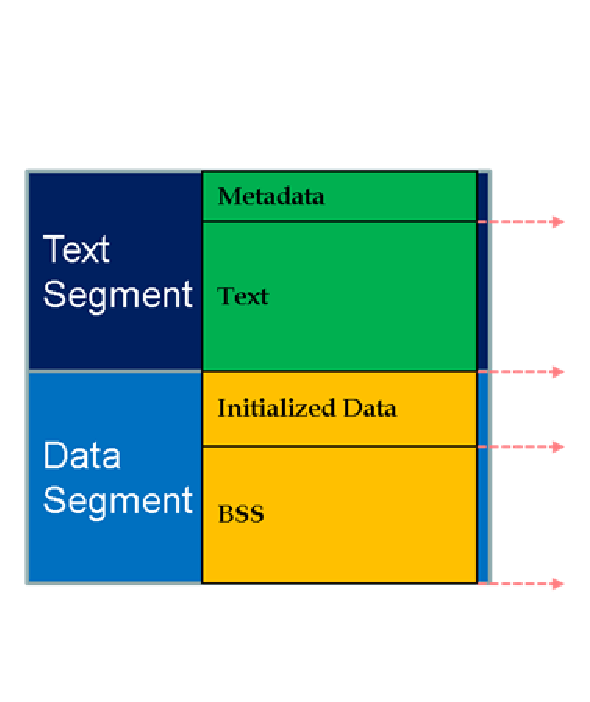
\includegraphics[scale=0.65]{executablep1.eps}
\label{Figure:OrigExecutable}
}
\subfigure[The structure of instrumented ELF file.]{
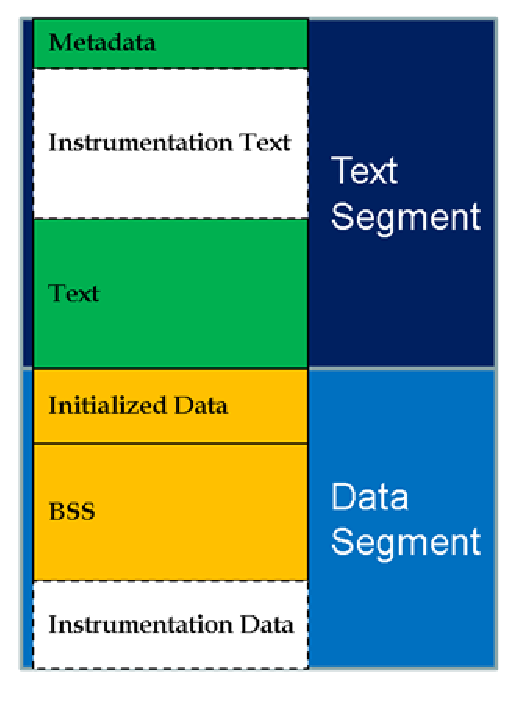
\includegraphics[scale=0.65]{executablep2.eps}
\label{Figure:InstExecutable}
}
\label{Figure:Executable}
\end{figure}

The instrumentation text contains several types of additional code. The first
contains code that accomplishes the instrumentation task as well as some code to
accompany it. When control is transferred from the application to the
instrumentation code, it is necessary to maintain the machine state of
the application in order to preserve its original behavior. This machine state
can contain anything modified by the instrumentation code, but in practice is
usually limited to a relatively limited set of registers but in some cases includes
some information about the call stack. The code snippet, called a \textit{trampoline} [CITE Dyninst], 
saves any machine state that will be destoryed, performs the instrumentation task, restores
the machine state after the instrumentation, executes the
original instructions that were displaced by the initial control transfer,
finally restoring control to the application. Since we are using a jump instruction at the instrumentation point, the
instrumentation code has no information about where control was transferred from
(as might be the case if we used a more heavyweight call instruction). Hence
each instrumentation point uses its own trampoline so that the location of the
instrumentation point can be hard-coded into an unconditional branch instruction
at the end of the trampoline.

Since some instrumentation tasks may need to include additional data for instrumentation code inserted,
PIX provides mechanisms to add and initialize additional data in to the executable.
The instrumentation text also includes code to initialize this additional data for use by the
instrumentation tool. Recall from Figure \ref{Figure:Executable} that the instrumentation
data was appended to the end of the application's data segment, after the
application's uninitialized data section  (BSS section). \textbf{(COMMENT: Let's say something why after BSS? I suppose
to reserve the original addresses in the code)} The initialized data and BSS
sections of the data segment are usually implemented by declaring the size of
the data segment in the executable to be smaller than the size of the data
segment in memory. According to the ELF[CITE] specification, the extra part of any
segment whose memory size is greater than its file size should be filled with
zeroes by the loader. Hence most programs just increase the size of the data
segment in memory by the size of the BSS section in order to get a large
area that is filled with zeroes and is reserved for uninitialized data. Since we
would like to use the area following the BSS section for additional
data for the instrumentation tool, we can either explicitly include the entire
segment's contents in the executable file or we can implicitly reserve this area
that is already in use by most programs.
Since the BSS section can be very large and explicit inclusion of its contents
would bloat the  executable file, we use the implicit
technique to reserve this section for instrumentation data. We therefore
temporarily store the instrumentation data with the instrumentation text in the
executable, as well as some code to copy it to the appropriate location in the
data segment once the program starts.


\label{Section:Efficiency}
\section{Efficiency}

The goal of PIX is to provide a toolkit that enables the construction of
instrumentation tools that produce an efficient instrumented
executable. More importantly, one of the design goals of PIX is to genearte efficient instrumented executables
when number of instrumentation points is rather high  In this section, we describe the mechanism used in PIX 
to produce efficient instrumented executables.

\label{Subsection:Relocation}
\subsection{Code Relocation at Function Level}
The use of relocation at the function level in PIX stems from the fact
that we are performing the instrumentation statically on a platform that uses a
variable-length instruction set and it may not be always possible to instrument
an arbitrary point in the executable due to the lack of enough space for jump instruction to the instrumentation code. 
A typical strategy used by static
instrumentation tools on platforms with fixed-length instruction sets is to
replace a single fixed-length instruction at the instrumentation point with a
branch instruction that will transfer control to the instrumentation code. This is fairly straightforward because by the
definition of a fixed-length instruction set, the instruction being replaced and
the replacing jump have the same length. 
%Performing static instrumentation in a variable-length instruction set does not afford us this luxury. 
In x86 platforms, a
jump instruction that uses a 32-bit offset requires 5 bytes. However, for some of
the instrumentation points of interest there may not be enough space to hold a 5 byte
jump instruction. This can occur in cases where a basic block or an instruction of interest
is smaller than 5 bytes. 

Figure \ref{Figure:InstructionSizes} shows a breakdown of the sizes of
instructions for many of the SPEC CPU2000 Integer benchmarks. This figure shows that for these benchmarks,
at least 52\% \textbf{(COMMENT: Let's put min-max range)} of instructions are smaller than 4 bytes. In fact, an average of 64\% \textbf{(COMMENT: Let's put min-max range)} of instructions
are smaller than the 5 bytes, which indicates that the the generic technique of replacing 
an instruction with a branch to instrumentation code deserves reexamination because without modification
this technique will not be able to provide instrumentation to large portions of the application code, especially 
if the instrumentation tool requires many instrumentation points.

\begin{figure}[ht]
\centering
\label{Figure:InstructionSizes}
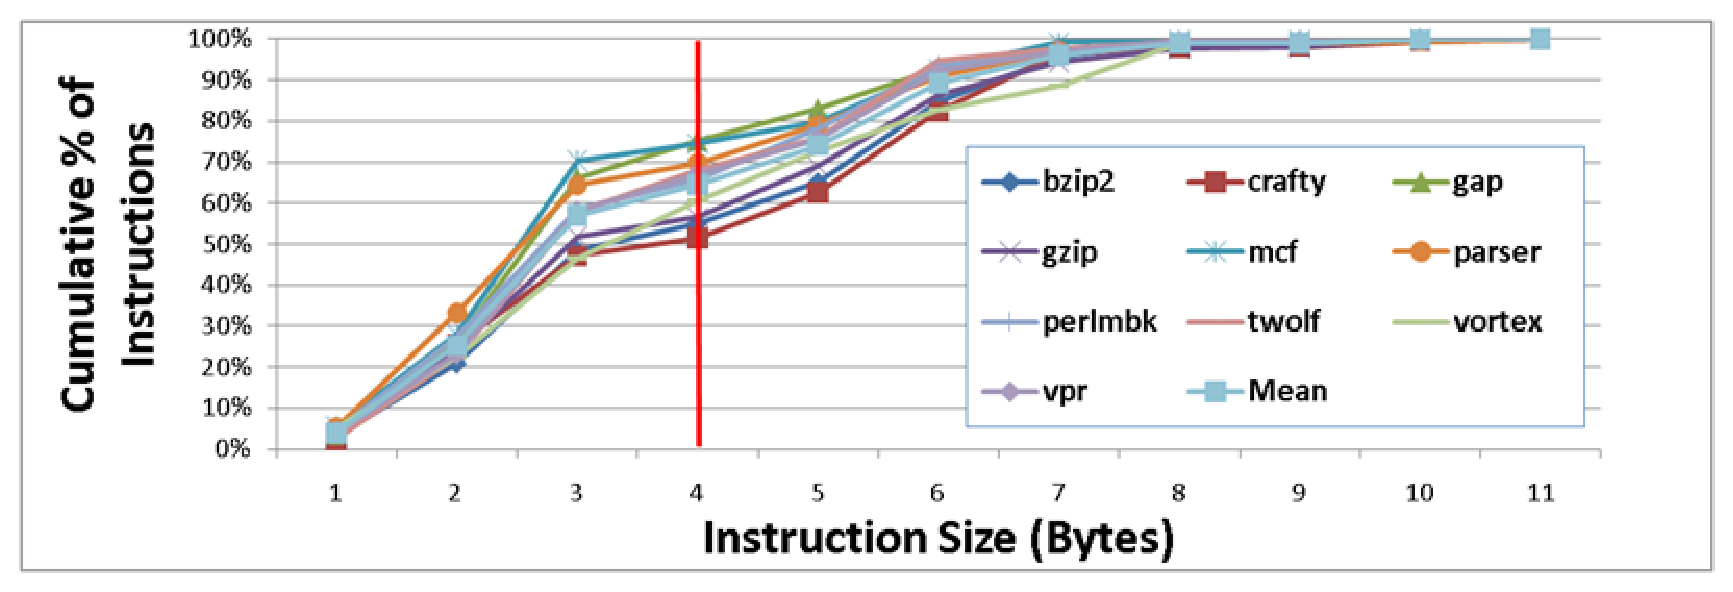
\includegraphics[scale=0.5]{instsize.eps}
\caption{Instruction sizes for several benchmarks presented in a cumulative basis.}
\end{figure}

This leaves two options for how to transfer control to the instrumentation code.
We must either use a technique entirely distinct from the idea of using a single
unconditional branch to execute the control transfer or we must somehow alter the application code so
that it can accommodate a single large control instruction that is larger than
the original amount of space available at the instrumentation point. One alternative
technique for transferring control flow could be to use a series of branches,
where the instruction in the instrumentation point is a small branch that
transfers control to a larger intermediate branch. This
method is unsatisfactory because the smallest traditional unconditional branch instruction available
on the x86 platform is 2 bytes in length, yet there are
instrumentation points with only a single byte available to them. \textbf{(COMMENT: Put the percetage of instruction under 2 bytes)}.
Besides, this technique would
require additional space to be available in close proximity to the instrumentation points since these
smaller branches are also very short reaching. 

Another option is the method proposed by the BIRD project \cite{nanda2006bird}, which
proposes the use of the single-byte \begin{it}INT3\end{it} instruction when a larger traditional
branch won't fit within the specified area. This instruction is functionally
perfect for static instrumentation because it consumes only a single byte and
allows us to transfer control to an arbitrary location by registering an
exception haThere will also be some overhead
associated with setting up a stack frame for the instrumentation function.ndler with the system. We performed a cursory study on this scheme
from an efficiency standpoint to determine whether it was worth further
investigation. On a small benchmark set, our implementation of using
\begin{it}INT3\end{it} only when 5-byte unconditional branches do not fit at
the instrumentation point introduces slowdown of at least 100X for
even a simple task of counting the number of executions of each basic block in the code. As one might
expect, this mechanism is unsuitable for efficient instrumentation since the
 heavyweight system call conventions are being invoked on a fairly regular basis.

In PIX, we use reorganization of the code at the function level so that
there is enough space at every instrumentation point to accommodate a 5-byte
jump. Specifically, the steps in whole function relocation includes \textit{function displacement}, \textit{linking function entry points},
\textit{branch conversion} and \textit{instruction padding}. Figure \ref{Figure:Relocation} presents the flow of information on 
this process with a simple example function in the original text section of an executable.

\begin{figure}[ht]
\centering
\caption[Optional caption for list of figures]
{The steps taken in order to prepare a function for instrumentation which collects
the memory addresses of an application.}
\subfigure[Original instruction sequence.]{
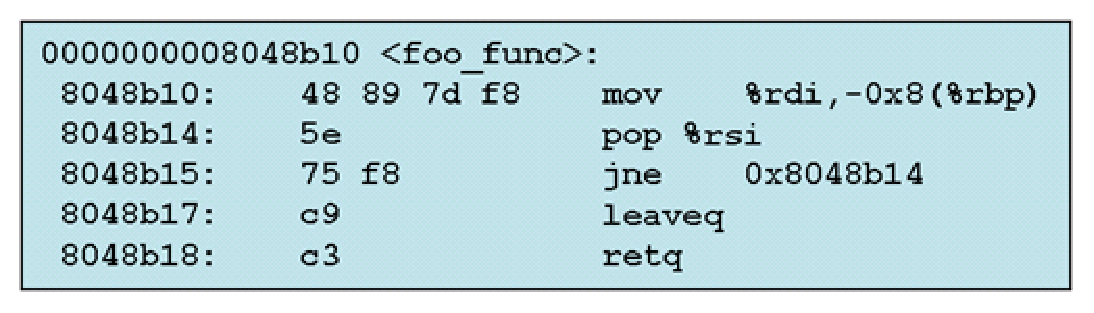
\includegraphics[scale=0.38]{funcp1.eps}
\label{Figure:funcp1}
}
\subfigure[Instructions after linking function entries.]{
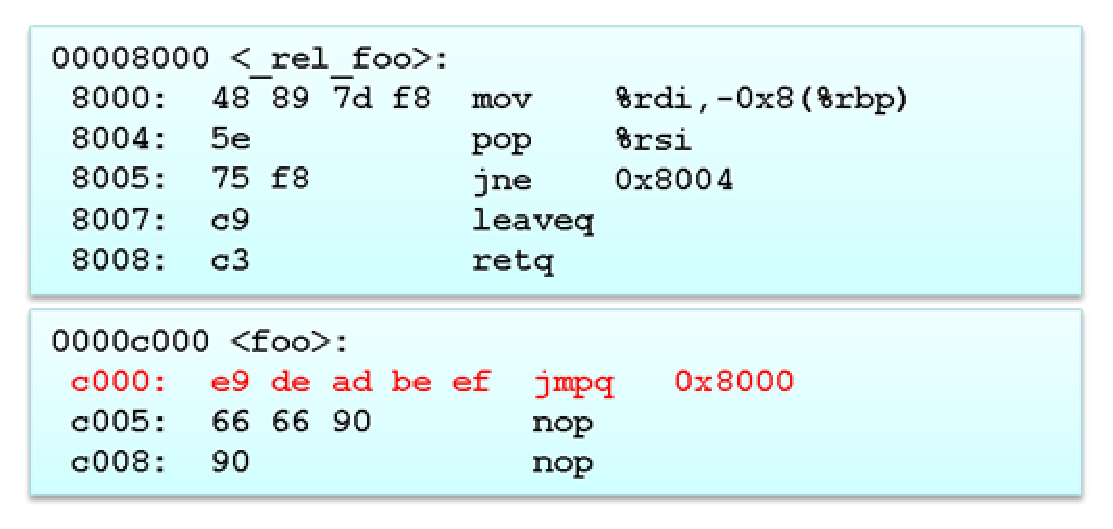
\includegraphics[scale=0.38]{funcp2.eps}
\label{Figure:funcp2}
}
\subfigure[Instructions after branch conversion.]{
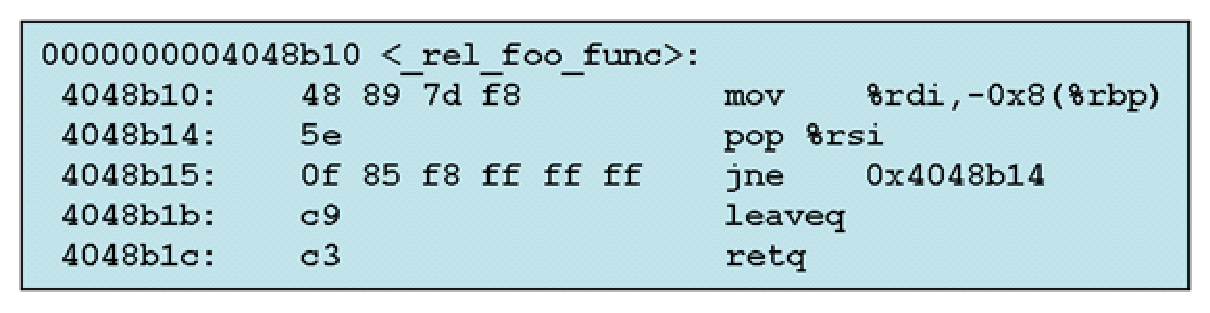
\includegraphics[scale=0.34]{funcp3.eps}
\label{Figure:funcp3}
}
\subfigure[Instructions after padding.]{
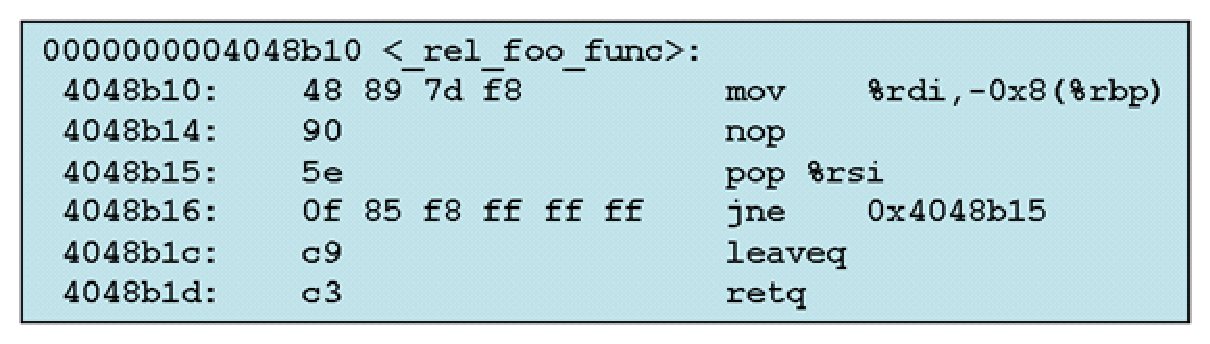
\includegraphics[scale=0.34]{funcp4.eps}
\label{Figure:funcp4}
}
\subfigure[Relocated function body.]{
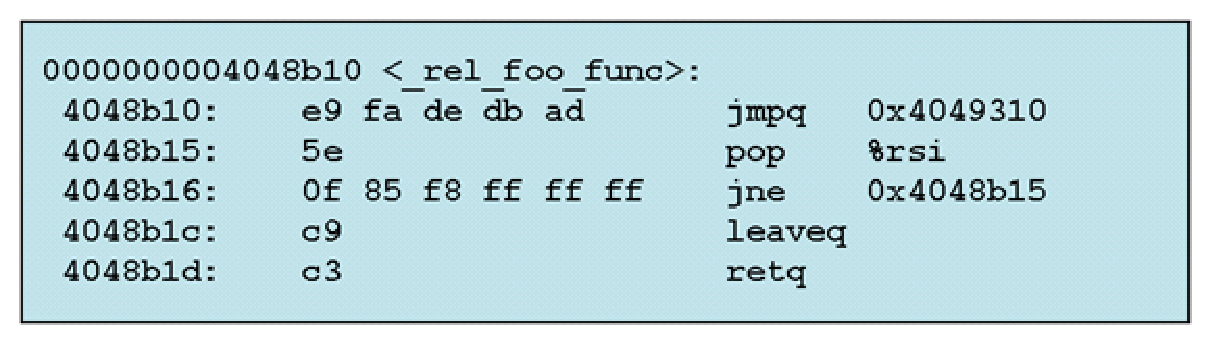
\includegraphics[scale=0.34]{funcp5.eps}
\label{Figure:funcp5}
}
\label{Figure:Relocation}
\end{figure}


\textit{Function Displacement} relocates the contents of the entire function to an area of the text section allocated
for the instrumentation. Since functions are often packed tightly together, it is generally not possible to
expand the size of a function without disturbing the entry points of another function using the original location of a function. 
\textit{Linking Function Entries} places an unconditional branch at the former function entry point that transfers control
to the new relocated function entry point. Most references to the entry point of a function are in the form of function calls, which
routinely are indirect references (i.e. their value is computed or looked up at runtime) and are difficult to resolve
prior to runtime. \textit{Branch Conversion} converts each short conditional branch in the relocated function to the equivalent
5-byte branch instruction. Since the code is being reorganized in the next step which may strain the limits of
smaller 8-bit or 16-bit offsets, we convert all branches to use 32-bit offsets so that the targets of each branch
will still be reachable without having the need to further reorganize the code. Note that there is opportunity
here to reduce space by using the smallest branch offset size that accommodates the branch, but we chose to use a single 
mechanism to simplify the implementation and optimize the space usage in the future. \textit{Instruction Padding} pads
the instruction at each instrumentation point with \begin{it}nop\end{it} instructions so that a 5-byte branch can fit
 according to the needs of the instrumentation. 

There are several ways that whole function relocation may adversely affect 
the performance of the instrumented executable independent of the overhead
that will be imposed by the additional instrumentation code. Each function call
now has an extra control interruption associated with it since control must be passed first to the original function entry
point and then to the relocated function entry point. In addition it is possible that using 32-bit offsets for every branch rather than
some smaller number of bits has an overhead associated with it. And since the code is being reorganized and expanded, 
we might destroy some positive alignment and size optimizations that the compiler might have made on the instructions in the
function.

To quantify the impact of whole function relocation and the other organizational changes we make
on the performance of applications, we show the results of experiments
where we generated executables in which functions are relocated and branches are converted to use 32-bit offsets, 
instruction padding is applied. This is basically the overhead of the transformations applied to the executable 
before any instrumentation code is inserted. We compared the performance of several applications to
the performance of the original executables. The overhead on the SPECINT 2000 benchmarks never exceeds 3.4\%, with an average
overhead of 0.8\%. Thus the basic overhead incurred by the code reorganization in PIX to accomodate all instrumentation points is
well within reason and does not represent a major hurdle for efficiency.

\subsection{Efficient Instrumentation Snippets}

In most instrumentation tools, the tasks accomplished by the instrumentation tool are accomplished by allowing the user
to transfer control from instrumentation points to the functions provided by the user, typically
via a shared library or some object code. Since these instrumentation functions are delivered via a shared library or other
object code, the instrumentation tool developer has the advantage to use a software devlepment toolchain and can
write the code in a language that compiles to the underlying object code. However, such delivery mechanism is heavyweight due to 
the overhead of a function invocation including saving the complete machine state for all possibles cases. In cases where
efficiency is important, it is more desirable to insert small sequences of assembly code to perform a task and only
save a small subset of machine state that will be affected rather than relying entirely on more heavyweight instrumentation functions.

Consider the example of an instrumentation point where we wish to increment a counter that resides in memory. 
In order to accompish this task with an instrumentation snippet, we transfer control to the
instrumentation point's trampoline which will save the flag registers, update the counter in memory, restore
the flags register, then transfer control back to the application. Using an instrumentation function, prior to performing
the task the trampoline must save the flag registers, any registers used by the function, and perform pushing an entry to the call stack.
This would also require at least 2 more jump instructions to enter and exit the instrumentation function. 
Furthermore these control flow transfers generally use the call/return paradigm, which in addition to changing the
application's program counter will also store and retreive information about the function call site onto the stack. 
The use of the instrumentation function is also more likely to pollute the instruction cache more than using a compact
instrumentation snippet. For an instrumentation snippet the application code must contend with the trampoline code
only, whereas using an instrumentation function puts the function code into contention with the other two as well. Hence, 
instrumentation functions tend to be more heaviweight solution, which would not be as appropriate when efficiency is considered
in instrumentation. Using simple snippets rather than instrumentation functions allows us to more efficiently gather 
asynchronous program information, which intuitively can be thought of as any information that could be dumped to
disk an processed offline. The Gao et. al. \cite{gao2005aliter} demostrates that using lightweight instrumentation snippets to buffer information
which is later processed by more heavyweight instrumentation functions in batches is an efficient yet entirely lossless way of processing asynchronous
program information. The avaialability of instrumentation snippets gives tool developers the flexibility to choose 
depending on their performance goals and software engineering needs.

% move this to overview section
The call stack during execution requires protection from the instrumentation code because compilers will often optimize a leaf function
by not explicitly creating a stack frame for the local function data to operate in. This optimization is safe for the application because during its
normal execution a leaf function will never call another function and thus its errant stack contents can never be smashed. In the case of an instrumentation
tool that calls an instrumentation function from a leaf, this guarantee no longer holds. Thus, the area above the stack needs to be protected when
an instrumentation function is called from a leaf function. During the disassembly of a function, PIX notes whether it is a leaf function (i.e. whether it contains any call
instructions). Later, during instrumentation, it automatically protects the stack contents for any instrumentation function calls that are made by
incrementing the stack pointer by a fixed safe amount, which has the effect of giving the leaf function a large stack frame while the instrumentation
function's stack frame uses the stack.


\label{Section:Results}
\section{Results}
%\section{Results}
\label{sec:Results}

The main design goal of PIX is to generate efficient instrumented code. 
To investigate the efficiency of instrumented executables created by PIX, we ran several experiments 
on a selection of benchmarks from the the SPEC CPU2000 Integer benchmark suite comprised of
bzip2, crafty, gap, gzip, mcf, parser, perlmbk, twolf, vortex and vpr. All of the experiments are run on a
single core of a quad-core 2.4GHz IA32 Intel Xeon running Red Hat Linux Enterprise 4.1.2 (Linux kernel 2.6.18). 

The first set of experiments quantifies the overhead of the program relocation and 
transformation techniques used by PIX and
described in Section \ref{Subsection:Relocation}. 
Recall that this technique adds an additional unconditional
branch execution to each function call in order to relocate the function, extends all of the branches in the code
to use 32-bit offsets, and pads each basic block whose size is fewer than 5 bytes with nops so that a
5 byte jump to the instrumentation code can be inserted. These transformations are performed on our benchmark set 
so that the code is ready for the insertion of instrumentation code but is not actually instrumented. 

Figure \ref{fig:RelocOverhead} presents
the runtime overhead seen in the instrumentation-ready executables as a percentage of the original application runtime.
The figure shows that the maximum overhead due to these modifications is 6.5\%, with an
average overhead of just 1.6\%. Among a set of popular dynamic instrumentation toolkits,
Pin, DynamoRIO and Valgrind, the lowest overhead for running the application within the instrumentation
tool but performing no instrumentation
on the IA32 platform is obtained by using DynamoRIO. DynamoRIO has an average of 38\% overhead and a maximum overhead of 113\% on
our SPEC CPU2000 Integer benchmark set \cite{luk2005pin}. This shows that the 
relocation and transformation method used by PIX has a minimal
performance impact on the performance of these benchmarks and thus is a suitable approach as a basis for
producing efficient instrumented code.

\begin{figure}[ht]
\centering
\label{fig:RelocOverhead}
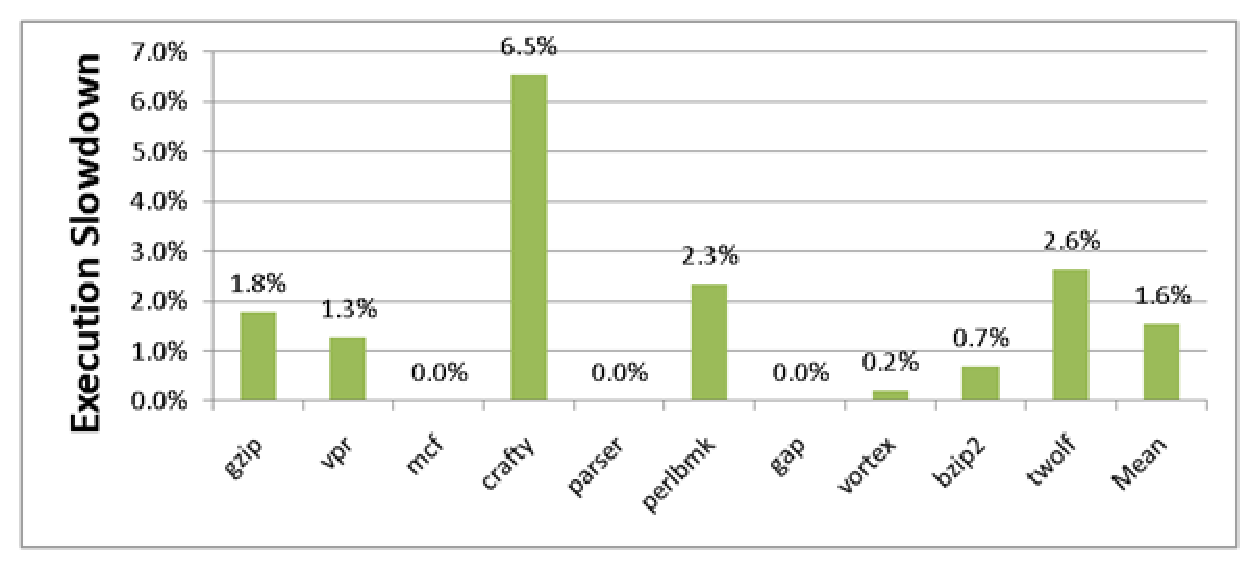
\includegraphics[scale=0.6]{relocperf.eps}
\caption{Application overhead caused by preparing the code for instrumentation but without
any instrumentation inserted.}
\end{figure}

The next set of experiments shows how much overhead is introduced due to counting the
basic block executions in the application. We use this particular instrumentation tool because basic block counting
is an example of an instrumentation tool where we would expect PIX to generate efficient instrumented executables
as the number of instrumentation points required is high. Much of the work performed in basic block counting, namely updating a single
counter every time a basic block is encountered, can be done easily using a fast instrumentation snippet rather than
by a full instrumentation function. The counters embodied in the instrumentation snippets must also be
persistent throughout the entire run of the application, which is more suited to a static instrumentation approach
because the static instrumentation does not utilize any resources to determine whether instrumentation can be removed.
The basic block counting instrumentation tool is used to produce an instrumented
executable for each program in our benchmark suite, whose runtime is compared to the runtime of the 
unmodified original executable. The results of these experiments are shown in Figure \ref{fig:ToolOverheads}. 

\begin{figure}[ht]
\centering
\label{fig:ToolOverheads}
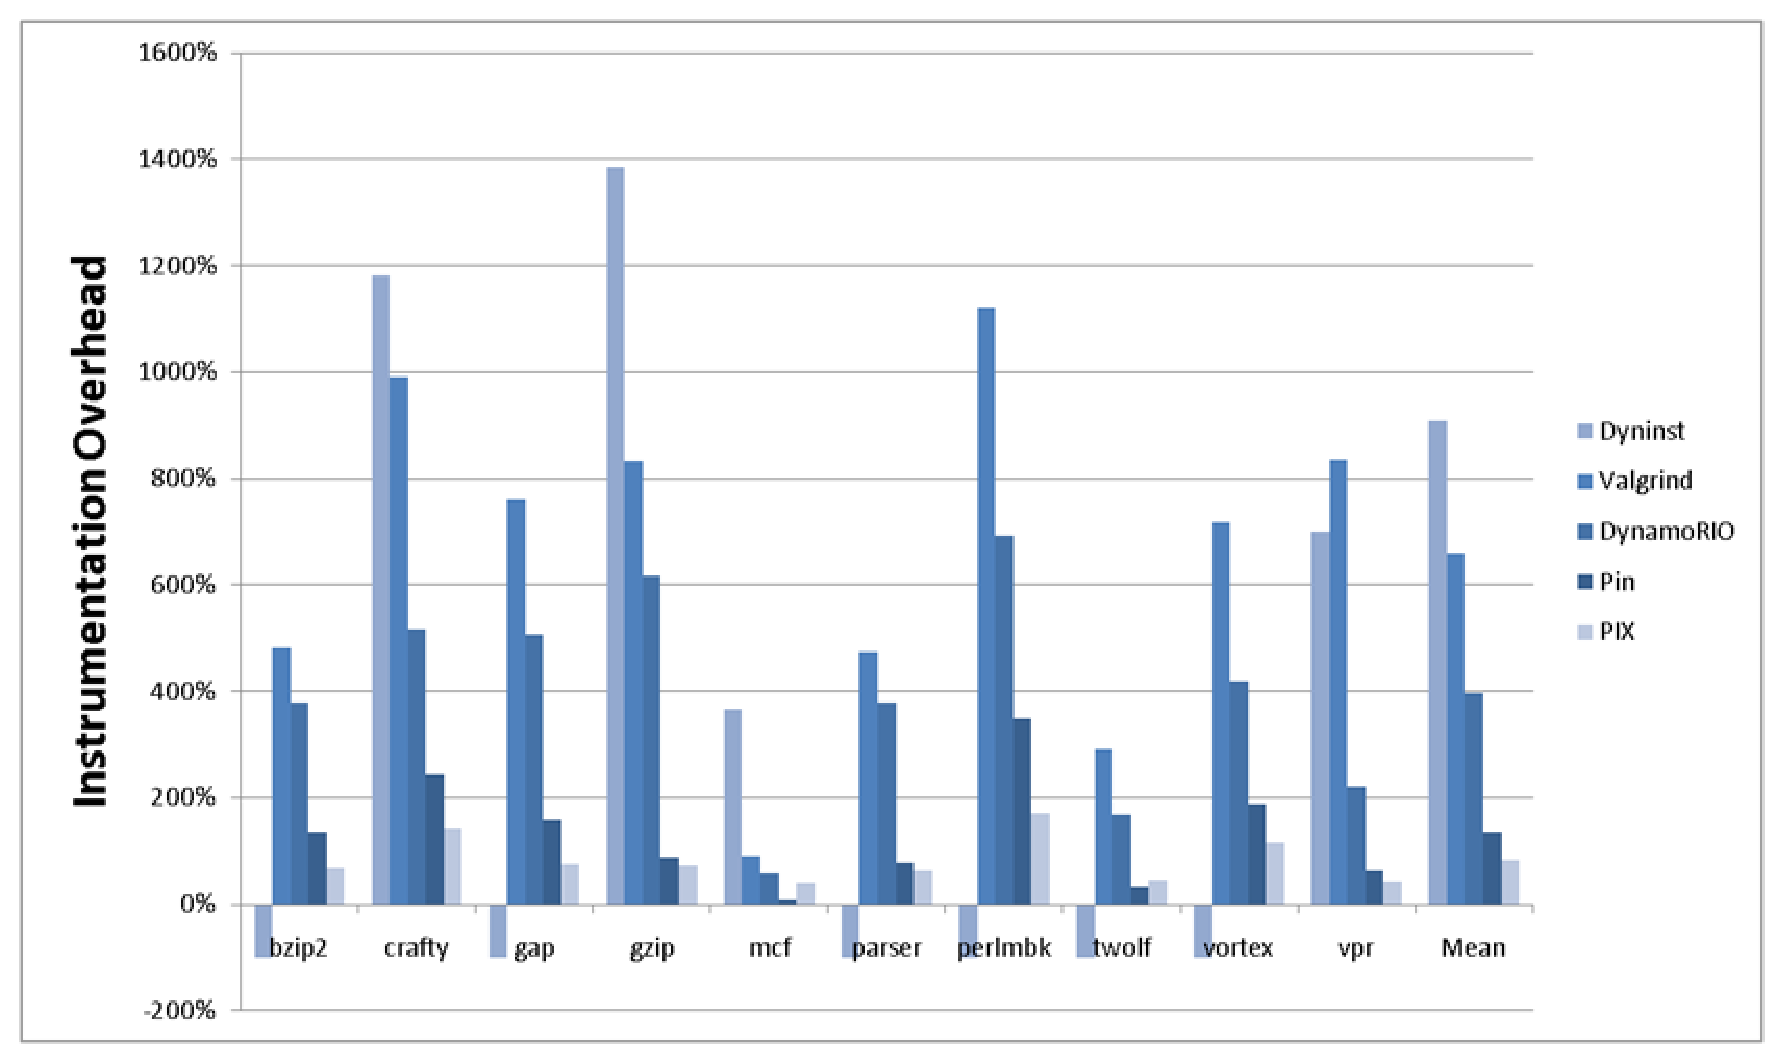
\includegraphics[scale=0.32]{bbcount.eps}
\caption{Performance of several x86 instrumentation tools with basic block counting instrumentation.}
\end{figure}

Figure \ref{fig:ToolOverheads} presents the overhead introduced as a percentage of the original application runtime. The
overhead of PIX's basic block counter ranges from 41\%-170\% for the benchmarks tested with an average overhead of 
84\%. More importantly, the figure shows that the overhead introduced by PIX instrumentation is significantly 
lower than those introduced by the other instrumentation toolkits available for the x86 platform. 
The average overhead is 135\% for Pin (ranging from 8\%-350\%), 
396\% for DynamoRIO (ranging from 58\%-693\%), 660\% for Valgrind (ranging from 91\%-1120\%), 
and 1936\% for Dyninst (ranging from 367\%-7859\%). Note also that, like PIX, the Dyninst
implementation of a basic block counter uses snippet-based instrumentation whenever possible yet
it results in significantly higher overheads than PIX.
Our experiments demonstrate that executables instrumented by PIX run an average of
51\% faster than the next most efficient instrumentation toolkit for basic block counting, Pin. Furthermore,
Pin uses a variety of optimizations such as tracking eflags bit liveness \cite{luk2005pin} that are currently
unincorporated into PIX. We plan to incorporate more optimizations to PIX in the future (see Section \ref{sec:Future}) including
several optimizations already in use by Pin, which should further improve the efficiency of the instrumented
executables generated by PIX.



\label{Section:Future}
\section{Future Work}
\label{sec:Future}

Despite the success in terms of efficiency, there are several additional techniques
that might make the instrumented code even more efficient in PIX. Because PIX relocates
the text to yeild extra space for the manipulation of the application functions, 
rather than inserting just a branch
that transfers control to the instrumentation code we have the opportunity to inline
the instrumentation code itsself
in order to reduce or eliminate the control interruptions  that otherwise must be taken 
when inserting the instrumentation code.

Currently PIX saves all general purpose registers around each function call and allows the
tool developer to state which registers are saved around instrumentation snippets. For even more efficient instrumentation
snippets, we could automatically detect which registers are killed by the instrumentation code and which are live at the entry point
of the instrumentation code, and automatically save only the ones that are alive. Similarly, we could perform register 
analysis in order to identify the instrumentation points where the machine state doesn't need to be saved around instrumentation functions. 

Finally, similar to Pin, we could perform liveness on the bits of the eflags/rflags register to determine whether the flag registers need to be saved and
restored at each instrumentation point. Optimizations that help PIX avoid saving and restoring state at each instrumentation point 
have the potential to further the overhead associated with instrumentation and we beleive 
that they will further the goal of generating efficient instrumented code with PIX.




\label{Section:Conclusions}
\section{Conclusions}
%\section{Conclusions}
\label{sec:Conclusions}


\bibliography{x86inst}
\bibliographystyle{unsrt}

\end{document}

